\begin{abox}
	Laplace Transforms
	\end{abox}

The Laplace transform $f(s)$ of a function $F(t)$ is defined by 
\begin{equation}
f(s)=\mathcal{L}\{F(t)\}=\int_{0}^{\infty} e^{-s t} F(t) d t .
\end{equation}
A few comments on the existence of the integral are in order. The infinite integral of $F(t)$,
\begin{equation*}
\int_{0}^{\infty} F(t) d t,
\end{equation*}
need not exist. For instance, $F(t)$ may diverge exponentially for large $t$. However, if there are some constants $s_{0}, M$, and $t_{0} \geq 0$ such that for all $t>t_{0}$
\begin{equation}
\left|e^{-s_{0} t} F(t)\right| \leq M,\label{LT-01}
\end{equation}
the Laplace transform will exist for $s>s_{0} $. $F(t)$ is then said to be of exponential order. As a counter example, $F(t)=e^{t^{2}}$ does not satisfy the condition given by Eq. (\ref{LT-01}) and is not of exponential order. Thus, $\mathcal{L}\left\{e^{t^{2}}\right\}$ does not exist.
The Laplace transform may also fail to exist because of a sufficiently strong singularity in the function $F(t)$ as $t \rightarrow 0$. For example,
\begin{equation*}
\int_{0}^{\infty} e^{-s t} t^{n} d t
\end{equation*}
diverges at the origin for $n \leq-1$. The Laplace transform $\mathcal{L}\left\{t^{n}\right\}$ does not exist for $n \leq-1$. Since, for two functions $F(t)$ and $G(t)$ for which the integrals exist,
\begin{equation}
\mathcal{L}\{a F(t)+b G(t)\}=a \mathcal{L}\{F(t)\}+b \mathcal{L}\{G(t)\}
\end{equation}
the operation denoted by $\mathcal{L}$ is linear.\\
\subsection{Important Laplace Transforms:}
\begin{enumerate}
	\item $L(1)=\frac{1}{s}$
	\item $L\left(x^{n}\right)=\frac{n !}{s^{n+1}}(n=0,1,2, \ldots \ldots . .)$
	\item $L\left(e^{a x}\right)=\frac{1}{s-a}(s>a)$
	\item $L(\cos a x)=\frac{s}{s^{2}+a^{2}}$
	$(s>0)$
	\item $L(\sin a x)=\frac{a}{s^{2}+a^{2}} \quad(s>0)$
	\item $L(\cosh a x)=\frac{s}{s^{2}-a^{2}}\left(s^{2}>a^{2}\right)$
	\item $L(\sinh a x)=\frac{a}{s^{2}-a^{2}}\left(s^{2}>a^{2}\right)$
\end{enumerate}

\subsubsection{Important properties:}
\begin{enumerate}
	\item Linear Property: $L\left[a_{1} f_{1}(x)+a_{2} f_{2}(x)\right]=a_{1} L\left[f_{1}(x)\right]+a_{2} L\left[f_{2}(x)\right]$
	\item Shifting Property: $L\left[e^{a x} f(x)\right]=f(s-a)$
	\item Scaling Property: $L[f(a x)]=\frac{1}{a} f\left(\frac{s}{a}\right)$
	\item $L\left[x^{n} f(x)\right]=(-1)^{n} \frac{d^{n}}{d s^{n}}(f(s))$
	\item $L\left[\frac{f(x)}{x}\right]=\int_{-\infty}^{\infty} f(s) d s$
	\item $L\left[\int_{0}^{t} f(x) d x\right]=\frac{1}{s} f(s)$
	\item $L\left[f^{\prime}(x)\right]=s L[f(x)]-f(0)$
	\item  $L\left[f^{\prime \prime}(x)\right]=s^{2} L[f(x)]-f^{\prime}(0)-s f(0)$
	\item Laplace transform of a periodic function $f(x)$ having period ' $T$ ' is $$L[f({x})]=\frac{1}{1-e^{-s T}} \int_{0}^{T} e^{-s x} f({x}) d {x}$$
	\item Laplace transform of the unit step function $u(x-a)=u_{a}(x)=\left\{\begin{array}{lll}0 & \text { for } & x<a \\ 1 & \text { for } & x \geq a\end{array}\right.$ is $\frac{e^{-a s}}{s}$.
	\item Laplace transform of the dirac delta function $\delta(x-a)$ is $e^{-a s}$.
\end{enumerate}
\begin{exercise}
	Find the laplace transform of $f(x)=(1+\cos 2 x)$
\end{exercise}
\begin{answer}
	\begin{align*}
	\begin{aligned}
	L[f(x)] &=\int_{0}^{\infty} e^{-s x}\left(1+\cos 2 x \cdot d x=\left(\frac{e^{-s x}}{-s}\right)_{0}^{\infty}+\int_{0}^{\infty} e^{-s x} \cos 2 x d x\right.\\
	&=\frac{1}{s}+\frac{s}{4+s}=\frac{2 s^{2}+4}{s\left(s^{2}+4\right)}
	\end{aligned}
	\end{align*}
\end{answer}
\begin{exercise}
	Find the laplace transform of $f(x)=2 \sin 2 x \cos 4 x$
\end{exercise}
\begin{answer}
	\begin{align*}
	L[f(x)]=L[2 \sin 2 x \cdot \cos 4 x]=L[\sin 6 x-\sin 2 x]=\left(\frac{6}{s^{2}+36}-\frac{2}{s^{2}+4}\right)
	\end{align*}
\end{answer}
\begin{exercise}
Find the laplace transform of $f(x)=e^{-x}(3 \sinh 2 x-5 \cosh 2 x)$
\end{exercise}
\begin{answer}
	\begin{align*}
	\begin{aligned}
	L[f(x)] &=L\left(3 e^{-x} \sinh 2 x\right)-L\left(5 e^{-x} \cosh 2 x\right) \\
	&=3 \frac{2}{(s+1)^{2}-4}-5 \cdot \frac{(s+1)}{(s+1)^{2}-4}=\frac{(1-5 \mathrm{~s})}{\left(\mathrm{s}^{2}+2 \mathrm{~s}-3\right)} \quad \text { (Using 2nd property) }
	\end{aligned}
	\end{align*}
\end{answer}
\begin{exercise}
	Find the laplace transform of the fuction\\
	$f(x)=1$ for $2 n \leq x \leq 2 n+1$\\
	$=0 \quad$ for $2 n+1 \leq x \leq 2 n+2 \quad(n=0,1,2, \ldots . .)$
\end{exercise}
\begin{answer}
	\begin{align*}
	L[f(x)] &=\frac{1}{1-e^{-s T}} \int_{0}^{T} e^{-s x} f(x) d x=\frac{1}{1-e^{-2 s}} \int_{0}^{2} e^{-s x} d x \\
	&=\frac{1}{1-e^{-2 s}}\left[\int_{0}^{1} e^{-s x} d x\right]=\frac{1}{1-e^{-2 s}}\left(\frac{1-e^{-s}}{s}\right)\\
	&=\frac{\left(1-e^{-s}\right)}{s\left(1+e^{-s}\right)\left(1-e^{-s}\right)}=\frac{1}{s\left(1+e^{-s}\right)}
	\end{align*}
\end{answer}
\begin{exercise}
	Find the laplace transform of $f(x)=\left(1+x e^{-x}\right)^{3}$
\end{exercise}
\begin{answer}
	\begin{align*}
	f(x)&=\left(1+x e^{-x}\right)^{3}=1+x^{3} e^{-3 x}+3 x e^{-x}+3 x^{2} e^{-2 x} \\
	L[f(x)]&=L(1)+L\left(x^{3} e^{-3 x}\right)+L\left(3 x e^{-x}\right)+L\left(3 x^{2} e^{-2 x}\right)\\
	&=\frac{1}{s}+(-1)^{3} \frac{d^{3}}{d s^{3}}\left(\frac{1}{s+3}\right)+3(-1)^{1} \frac{d}{d s}\left(\frac{1}{s+1}\right)+3(-1)^{2} \frac{d^{2}}{d s^{2}}\left(\frac{1}{s+2}\right)\text{ (Using 4th property)}\\
	&=\frac{1}{s}+\frac{6}{(s+3)^{4}}+\frac{3}{(s+1)^{2}}+\frac{6}{(s+2)^{3}} \text {. }
	\end{align*}
\end{answer}
\begin{exercise}
	Find the laplace transform of $f(x)=\frac{1-e^{x}}{x}$
\end{exercise}
\begin{answer}
	\begin{align*}
	L\left(\frac{1-e^{x}}{x}\right)&=\int_{s}^{\infty}\left(\frac{1}{s}-\frac{1}{s-1}\right) d s=[\ln s-\ln (s-1)]_{s}^{\infty}=\left[\ln \frac{s}{s-1}\right]_{s}^{\infty}:\text{ (Using 5th property)}\\
	&=[\ln s-\ln (s-1)]_{s}^{\infty}=\left[\ln \frac{s}{s-1}\right]_{s}^{\infty}=\ln \left(\frac{1}{\left.1-\frac{1}{s}\right)_{s}}\right)^{\infty} \\
	&=0-\ln \frac{s}{s-1}=\ln \frac{(s-1)}{s}
	\end{align*}
\end{answer}
\begin{exercise}
	Find the inverse laplace transform of
	$$\mathrm{f}(\mathrm{s}) =\frac{\mathrm{s}-2}{(\mathrm{~s}-2)^{2}+25}+\frac{\mathrm{s}+4}{(\mathrm{~s}+4)^{2}+81}+\frac{1}{(\mathrm{~s}+2)^{2}+9} $$
\end{exercise}
\begin{answer}
	\begin{align*}
	\mathrm{~L}^{-1}[\mathrm{f}(\mathrm{s})] &=\mathrm{L}^{-1}\left[\frac{\mathrm{s}-2}{(\mathrm{~s}-2)^{2}+25}\right]+\mathrm{L}^{-1}\left[\frac{\mathrm{s}+4}{(\mathrm{~s}+4)^{2}+81}\right]+\mathrm{L}^{-1}\left[\frac{1}{(\mathrm{~s}+2)^{2}+9}\right] \\
	&=\mathrm{e}^{2 \mathrm{x}} \cos 5 \mathrm{x}+\mathrm{e}^{-4 \mathrm{x}} \cos 9 \mathrm{x}+\frac{\mathrm{e}^{-2 \mathrm{x}}}{3} \sin 3 \mathrm{x}
	\end{align*}
\end{answer}
\begin{exercise}
	The graph of the function
	$$f(x)= \begin{cases}1 & \text { for } 2 n \leq x \leq 2 n+1 \\ 0 & \text { for } 2 n+1 \leq x \leq 2 n+2\end{cases}$$
	(Where $n=0,1,2,........$)is shown below.
	\begin{figure}[H]
		\centering
		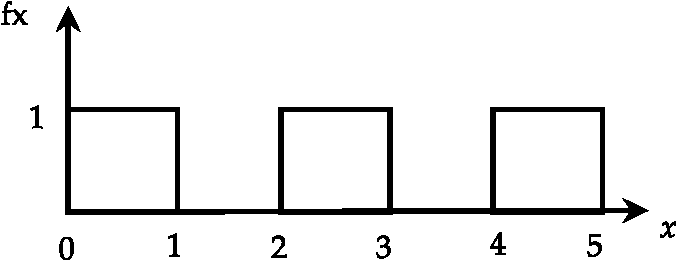
\includegraphics[height=2.5cm,width=6cm]{LT-01}
	\end{figure}
	Its Laplace transform $\tilde{f}(\mathrm{s})$ is
	 \begin{tasks}(2)
		\task[\textbf{a.}]$\frac{1+e^{-s}}{s}$
		\task[\textbf{b.}]$\frac{1-e^{-s}}{s}$
		\task[\textbf{c.}]$\frac{1}{s\left(1+e^{-s}\right)}$
		\task[\textbf{d.}]  $\frac{1}{s\left(1-e^{-s}\right)}$
	\end{tasks}
\end{exercise}
\begin{answer}
	Given function is a periodic function of period $T=2$
	\begin{align*}
	L[f(x)] &=\frac{1}{1-e^{-s T}} \int_{0}^{T} e^{-s x} f(x) d x=\frac{1}{1-e^{-2 s}} \int_{0}^{2} e^{-s x} d x \\
	&=\frac{1}{1-e^{-2 s}}\left[\int_{0}^{1} e^{-s x} d x\right]=\frac{1}{1-e^{-2 s}}\left(\frac{1-e^{-s}}{s}\right) \\
	&=\frac{\left(1-e^{-s}\right)}{s\left(1+e^{-s}\right)\left(1-e^{-s}\right)}=\frac{1}{s\left(1+e^{-s}\right)}
	\end{align*}
	So the correct answer is \textbf{option (c)}
\end{answer}
\begin{exercise}
	The inverse transform of $\frac{1}{s^2(s+1)}$ is
	 \begin{tasks}(2)
		\task[\textbf{a.}]$\frac{1}{2} t^{2} e^{-t}$
		\task[\textbf{b.}]$\frac{1}{2} t^{2}+1-e^{-t}$
		\task[\textbf{c.}]$t-1+e^{-t}$
		\task[\textbf{d.}] $\frac{1}{2} t^{2}\left(1-e^{-t}\right)$ 
	\end{tasks}
\end{exercise}
\begin{answer}
	\begin{align*}
	&f(s)=\frac{1}{s^{2}(s+1)}=\frac{(s+1)-s(s+1)+s^{2}}{s^{2}(s+1)}=\frac{1}{s^{2}}-\frac{1}{s}+\frac{1}{s+1} \\
	&\Rightarrow L^{-1}[f(s)]=t-1+e^{-t}
	\end{align*}
		So the correct answer is \textbf{option (c)}
\end{answer}
